% Source: Code/xband-radar-sim/docs/radar_simulation_technical.tex
% Description: Polar to Cartesian scan conversion. Bilinear interpolation fills gaps in the Cartesian grid.

\documentclass[border=4pt]{standalone}
\usepackage{algpseudocode}
\usepackage{amsmath,amssymb,amsfonts}
\usepackage[T1]{fontenc}
\usepackage{graphicx}
\usepackage{pgfplots}
\usepackage{tikz}
\usepackage{xcolor}
\pgfplotsset{compat=1.18}
\usetikzlibrary{arrows.meta,positioning,shapes.geometric,calc,patterns,decorations.pathmorphing,3d,angles,quotes}

\definecolor{radargreen}{RGB}{0,255,0}
\definecolor{raycolor}{RGB}{255,165,0}
\definecolor{targetcolor}{RGB}{255,0,0}
\definecolor{groundcolor}{RGB}{139,90,43}
\definecolor{skycolor}{RGB}{135,206,235}
\definecolor{beamcolor}{RGB}{255,255,0}


\begin{document}
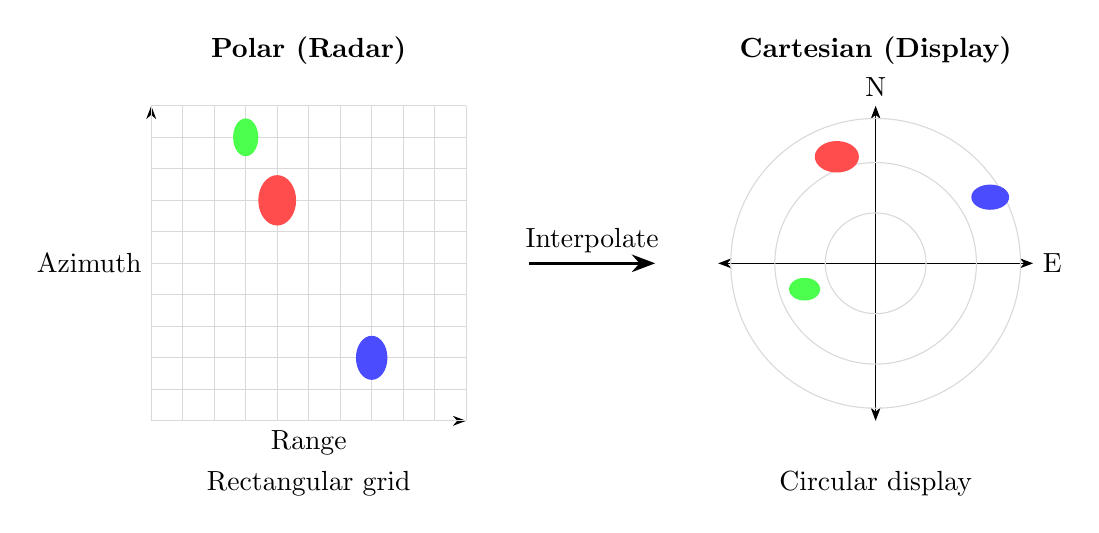
\begin{tikzpicture}[scale=0.8]
    % Polar representation
    \begin{scope}[shift={(0,0)}]
        \node[above] at (2.5,5.5) {\textbf{Polar (Radar)}};

        \draw[{Stealth}-{Stealth}] (0,5) -- (0,0) -- (5,0);
        \node[below] at (2.5,0) {Range};
        \node[left] at (0,2.5) {Azimuth};

        % Grid
        \draw[gray!30, step=0.5] (0,0) grid (5,5);

        % Target blobs in polar
        \fill[red!70] (2,3.5) ellipse (0.3 and 0.4);
        \fill[blue!70] (3.5,1) ellipse (0.25 and 0.35);
        \fill[green!70] (1.5,4.5) ellipse (0.2 and 0.3);

        \node at (2.5,-1) {Rectangular grid};
    \end{scope}

    % Arrow
    \draw[-{Stealth}, very thick] (6,2.5) -- (8,2.5) node[midway, above] {Interpolate};

    % Cartesian representation
    \begin{scope}[shift={(9,0)}]
        \node[above] at (2.5,5.5) {\textbf{Cartesian (Display)}};

        \draw[{Stealth}-{Stealth}] (0,2.5) -- (5,2.5);
        \draw[{Stealth}-{Stealth}] (2.5,0) -- (2.5,5);
        \node[right] at (5,2.5) {E};
        \node[above] at (2.5,5) {N};

        % Range rings
        \draw[gray!30] (2.5,2.5) circle (0.8);
        \draw[gray!30] (2.5,2.5) circle (1.6);
        \draw[gray!30] (2.5,2.5) circle (2.3);

        % Target blobs in Cartesian (transformed)
        \fill[red!70] ($(2.5,2.5)+(110:1.8)$) ellipse (0.35 and 0.25);
        \fill[blue!70] ($(2.5,2.5)+(30:2.1)$) ellipse (0.3 and 0.2);
        \fill[green!70] ($(2.5,2.5)+(200:1.2)$) ellipse (0.25 and 0.18);

        \node at (2.5,-1) {Circular display};
    \end{scope}
\end{tikzpicture}
\end{document}
